%% DONE
\id{МРНТИ \href{https://grnti.ru/?p1=06&p2=61&p3=23}{06.61.23}: \href{https://grnti.ru/?p1=06&p2=71&p3=07}{06.71.07}}{https://doi.org/10.58805/kazutb.v.1.26-733}

\begin{articleheader}
\sectionwithauthors{Б.У. Сыздыкбаева}{МЕТОДИКА ПРОЕКТИРОВАНИЯ РАЗМЕЩЕНИЯ ЛОГИСТИЧЕСКОЙ ИНФРАСТРУКТУРЫ АГРОПРОДОВОЛЬСТВЕННОЙ ПРОДУКЦИИ}

{\bfseries
Б.У. Сыздыкбаева\textsuperscript{\envelope } \alink{https://orcid.org/0000-0001-9463-4933}}
\end{articleheader}

\begin{affiliation}
\emph{Евразийский национальный университет им. Л.Н. Гумилева, Астана, Казахстан}

\raggedright \textsuperscript{\envelope }{\em Корреспондент-автор: \href{mailto:bakyt_syzdykbaeva@mail.ru}{\nolinkurl{bakyt\_syzdykbaeva@mail.ru}}}
\end{affiliation}

Выбор оптимального места размещения логистической инфраструктуры
способствует повышению качества, безопасности продукции и уровня
удовлетворенности потребителей, снижению затрат.

В статье рассматривается методологический подход к формированию и
определению потенциальных мест размещения логистической инфраструктуры:
складских хранилищ, оптово-распределительных центров по хранению, сбыту
и торговле агропродовольственной продукцией на территории страны, а
также предполагаемых зон их обслуживания, способствующих повышению
эффективности их функционирования.

Предлагаемый подход, в отличие от существующих ранее, учитывает
особенности функционирования инфраструктуры хранения, сбыта и торговли,
взаимоувязывает эти объекты с транспортной и складской доступностью на
территории регионов.

Предлагаемая методика позволяет определить потенциальные характеристики
логистической инфраструктуры по хранению продукции в зависимости от
выделенных критериев; потенциальные места размещения и количество
региональных логистических инфраструктур по хранению, сбыту и торговле,
а также зоны их обcлуживания с учетом их функционального назначения.
Является источником важной информации в процессе проектирования
логистической инфраструктуры, проведения дифференцированной
инвестиционной политики при ее строительстве и эксплуатации.

{\bfseries Ключевые слова:} методологический подход, логистическая
инфраструктура, критерий выбора и размещения, социальные факторы,
экономические факторы, инфраструктурно-географические факторы,
производственные факторы, экологические факторы.

\begin{articleheader}
{\bfseries АУЫЛ ШАРУАШЫЛЫҒЫ ӨНІМДЕРІНІҢ ЛОГИСТИКАЛЫҚ ИНФРАҚҰРЫЛЫМЫН ОРНАЛАСТЫРУДЫ ЖОБАЛАУ ӘДІСТЕМЕСІ}

{\bfseries
Б.Ұ. Сыздықбаева\textsuperscript{\envelope }}
\end{articleheader}

\begin{affiliation}
\emph{Л.Н. Гумилев атындағы Еуразиялық ұлттық университеті, Астана қ., Қазақстан,}

\emph{e-mail: \href{mailto:bakyt_syzdykbaeva@mail.ru}{\nolinkurl{bakyt\_syzdykbaeva@mail.ru}}}
\end{affiliation}

Логистикалық инфрақұрылым үшін оңтайлы орынды таңдау сапаны, өнімнің
қауіпсіздігін, тұтынушылардың қанағаттану деңгейін арттыруға және
шығындарды азайтуға көмектеседі.

Мақалада логистикалық инфрақұрылымның: ауыл шаруашылығы өнімдерін сақтау
қоймалары, сақтау, өткізу және саудалау көтерме-тарату орталықтарының
ықтималды орындарын қалыптастыру мен анықтаудың әдіснамалық тәсілі,
сондай-ақ олардың жұмыс істеу тиімділігін арттыруға ықпал ететін қызмет
көрсету аймақтары қарастырылады.

Ұсынылып отырған тәсілдің бұрын қолданылып жүргендерден айырмашылығы,
сақтау, өткізу және сауда инфрақұрылымының қызмет ету ерекшеліктерін
ескереді және бұл объектілерді өңірлердегі көліктік және қоймалық
қолжетімділікпен өзара байланыстырады.

Ұсынылған әдістеме таңдалған критерийлерге байланысты өнімдерді сақтауға
арналған логистикалық инфрақұрылымның әлеуетті сипаттамаларын анықтауға;
сақтауға, өткізуге және саудалауға арналған өңірлік логистикалық
инфрақұрылымдардың әлеуетті орындары мен санын анықтауға, сондай-ақ
олардың функционалдық мақсатын ескере отырып, олардың қызмет көрсету
аймақтарын анықтауға мүмкіндік береді. Ол логистикалық инфрақұрылымды
жобалау, оны салу және пайдалану кезінде сараланған инвестициялық
саясатты жүзеге асыру процесінде маңызды ақпарат көзі болып табылады.

{\bfseries Түйін сөздер:} әдістемелік тәсіл, логистикалық инфрақұрылым,
таңдау және орналастыру критерийлері, әлеуметтік факторлар, экономикалық
факторлар, инфрақұрылымдық-географиялық факторлар, өндірістік факторлар,
экологиялық факторлар

\begin{articleheader}
{\bfseries METHODOLOGY FOR DESIGNING THE PLACEMENT OF LOGISTICS INFRASTRUCTURE FOR AGRI-FOOD PRODUCTS}

{\bfseries
B.U. Syzdykbayeva\textsuperscript{\envelope }}
\end{articleheader}

\begin{affiliation}
\emph{L.N. Gumilyov Eurasian National University, Astana, Kazakhstan,}

\emph{e-mail: \href{mailto:bakyt_syzdykbaeva@mail.ru}{\nolinkurl{bakyt\_syzdykbaeva@mail.ru}}}
\end{affiliation}

Choosing the optimal location of the logistics infrastructure helps to
improve the quality, safety of products and the level of customer
satisfaction and contributes to cost reduction.

The article considers a methodological approach to the formation and
identification of potential locations of logistics infrastructure:
warehouse storage facilities, wholesale distribution centers for
storage, marketing and trade of agri-food products in the country, as
well as their intended service areas that contribute to improving the
efficiency of their functioning.

The proposed approach, as opposed to previous ones, takes into account
the specifics of the functioning of the storage, sales and trade
infrastructure, and connects these objects with transport and warehouse
availability in the regions.

The proposed methodology allows us to determine the potential
characteristics of the logistics infrastructure for storing products
depending on the selected criteria; potential locations and the number
of regional logistics infrastructures for storage, sales and trade, as
well as their service areas, taking into account their functional
purpose. It is a source of important information in the process of
designing logistics infrastructure, conducting a differentiated
investment policy during its construction and operation.

{\bfseries Keywords:} methodological approach, logistics infrastructure,
selection and placement criteria, social factors, economic factors,
infrastructural and geographical factors, production factors,
environmental factors

\begin{multicols}{2}
{\bfseries Введение.} Решение проблемы оптимального размещения и зоны
обслуживания логистических инфраструктур по хранению, сбыту и торговле
агропромышленной продукцией по территории страны и их эффективной работы
является актуальной для Казахстана.

Несмотря на многочисленные научные разработки по выбору места размещения
распределительных центров (РЦ) для сбыта агропродовольственной продукции
и их проектирования, а также оценки эффективности их деятельности, можно
констатировать, что имеющиеся решения научной проблемы в области
организационно-методического обеспечения формирования логистической
инфраструктуры требуют более обстоятельного изучения, в особенности,
применительно к сельскохозяйственной продукции.

Цель исследования - разработка методических решений по
формированию и эффективному размещению логистической инфраструктуры по
хранению, сбыту и торговле агропродовольственной продукцией, в
частности, складских хранилищ и оптово-распределительных центров (ОРЦ).

Методика позволяет проектировать и определять места размещения ОРЦ на
территории с учетом транспортных сетей и транзитного потенциала, а также
региональных факторов (социально-экономических, экологических,
производственных). В настоящее время такая методика отсутствует.
Предполагаемые места размещения и предлагаемая мощность описаны в
различных документах по развитию агропромышленного комплекса (АПК) и
торговли Казахстана. Однако, в них отсутствуют методические подходы,
методика и рекомендации по развитию логистической инфраструктуры по
регионам.

Предлагаемый метод может быть использован как логистическими
провайдерами для анализа и выбора оптимального места размещения
логистического центра с учетом существующей клиентской базы, владельцами
агропромышленных и транспортных зон, находящихся непосредственно на
территории крупных регионов, так и государственными органами для
планирования размещения логистических инфраструктур по территории
страны.

{\bfseries Материалы и методы.} \emph{А. Методология создания и размещения
логистической инфраструктуры оптово-распределительных центров
агропродовольственной продукции.}

Проведенный анализ научной литературы позволил выявить значительное
количество работ, в которых предложены математические модели и методы
определения месторасположения сетей складов и транспортно-логистических
терминалов, логистических центров (ЛЦ) на территории региона.

В настоящее время разработано множество методов решения задачи
оптимального размещения складского терминала, среди которых можно
выделить метод полного перебора, эвристический метод, метод центра
тяжести, экономико-математические модели.

Анализ показывает, что при планировании и определении местоположения
логистических или распределительных центров наиболее широко используются
следующие методы и их смешанные модели: модель целочисленного
программирования {[}1{]}, методика предпочтения заказов {[}2{]}, метод
теории гравитации, многоцелевая оптимизационная модель, метод
кластеризации K-средних {[}3{]}, метод AHP (Процесс нечеткой
аналитической иерархии), метод нечеткой комплексной оценки {[}4{]},
ГИС-технологии {[}5{]}, P-медианная модель {[}6{]}, интегрированная
модель производства и распределения агропродукции {[}7{]}.

Указанные исследования решают задачу определения и размещения ЛЦ. Не
умаляя достоинств каждого из вышеперечисленных методов, следует
отметить, что, с одной стороны, данные методы требуют использования
множества показателей (процесс сбора, обработки и вычисления - очень
трудоемкий), многие методы дают приближенные оценку. С другой стороны,
не учтены факторы, учитывающие привязки ЛЦ к конкретным географическим и
территориальным образованиям. Кроме этого, в них не предусмотрена
взаимная увязка местоположения транспортной и логистической
инфраструктуры на территории страны.

В методологии проектирования распределительной сети важным элементом
является формирование ее структуры, определение количества эшелонов и
для каждого эшелона - типа, размера, количества и расположения объектов,
где продукт временно хранится на пути к клиенту {[}8{]}. Вопрос
проектирования разнообразных распределительных сетей и выбор из них
оптимальных вариантов состоит из трех этапов {[}9{]}: 1)генерация
вариантов конфигурации и предварительная оценка; 2)количественная оценка
созданных вариантов; 3)детальное проектирование и точная настройка.

Вопросы проектирования распределительной и складской сети для
продовольственного рынка рассмотрены в работах {[}10-14{]}. В указанных
работах на первоначальном этапе оценивалась привлекательность региона на
основе ключевых социально-экономических факторов, выбор участка для РЦ.
На втором этапе строилась целевая функция, минимизирующая суммарные
затраты, связанные с перемещением товаров от поставщиков до конечных
потребителей с использованием методов дискретной оптимизации.
Проектирование сельскохозяйственного РЦ {[}15{]} состоит в изучении зоны
обслуживания и выбора участка под его создание. Попов П. В., Мирецкий И.
Ю. {[}16{]} выделяют два этапа в формировании логистических
инфраструктуры регионов: определение районов, где целесообразно
размещение объектов логистической инфраструктуры; привязка объектов на
местности и определение их мощности и вида транспортных средств.

В работе {[}17{]} предложена двухэтапная модель планирования для
размещения центров сбора продуктов для ЛЦ на основе двух моделей.
Детерминированная модель определяет места расположения центров сбора
продукции. Стохастическая модель определяет потенциальные места сбора
продукции с учетом факторов окружающей среды и риска.

Выбор местоположения ЛЦ проведен с помощью методов многокритериального
принятия решений на основе ранжирования предпочтений для критериев с
учетом различных сценариев, в которых используются весовые коэффициенты
критериев {[}18{]}. Анализ показал наличие эффективности при совместном
использовании предложенных методов.

Местоположение ЛЦ влияет на экономическую, социальную и экологическую
устойчивость городской логистики {[}19{]}. Так, время в пути,
транспортные расходы, выбросы углерода варьируются от расстояния ЛЦ до
центра города, что требует планирования маршрутов движения транспорта.
На выбор конфигурации и на процесс проектирования логистической сети
влияет сезонность поставок скоропортящихся продуктов {[}20{]}.

В указанных исследованиях процесс проектирования ЛЦ осуществляется для
конкретных товаров или группы товаров, или ЛЦ с узкими функциональными
назначениями, тогда как распределение, хранение и торговля
продовольственной продукцией имеет свои особенности (широкий ассортимент
товаров), которые нужно учитывать при определении места их размещения в
зависимости от их функционального назначения объектов хранения,
распределения и торговли.

Применяемые на практике модели и методы определения оптимального
месторасположения объектов логистической инфраструктуры дают
приближенное решение. Кроме того, в них не предусмотрен процесс
формирования взаимоувязанных складской и транспортной инфраструктуры на
территории региона.

Можно заключить, что в литературе нет единого мнения относительно этапов
процесса проектирования, выбора и использования показателей,
определяющих места размещения объектов, к которым следует оптимально
следовать (предписывающие) при принятии решения о выборе элементов и
структуры хранения или распределения. Также оспариваются начало процесса
и его последовательность.

Вклад нашего исследования заключается в комбинированном использовании
разных методов на разных этапах исследования. Применение метода
стандартизации показателей, кластерного анализа, регрессионного анализа,
факторного анализа, метода центра тяжести, метода ранжирования регионов
по выделенным нами критериям для выбора типа ОРЦ позволяет разработать
более практичный способ уточнения количества ОРЦ, что позволяет
учитывать факторы спроса на ОРЦ по регионам. Данный метод, с учетом
предлагаемых факторов, позволит избежать строительства невостребованных
ОРЦ.

Еще одной особенностью предлагаемого методического подхода является
построение взаимоувязанной транспортной и логистической инфраструктуры
на территории региона.

По нашему мнению, предложенный вариант позволит существенно повысить
эффективность использования транспортно-логистической инфраструктуры в
регионах в соответствии их потребностям на основе учета
социально-экономических, географических, экологических, производственных
факторов и требований. Выполнение данных требований позволит кардинально
повысить процесс создания и реализации потребительской ценности ОРЦ:
системно предоставлять клиенту именно то, чего он хочет, в нужное ему
время и~удобном для него месте.

Таким образом, распределение, хранение и торговля агропродовольственной
продукцией в цепях поставок имеют свои особенности, которые нужно
учитывать при определении места их размещения в зависимости от их
функционального назначения объектов хранения, распределения и торговли.

Поэтому с точки зрения оптимальности и эффективности функционирования
системы хранения, распределения и торговли продукцией справедливым
остается одно требование: формирование системы показателей, дающей
оценку всех включенных в ее состав функций аграрного сектора, торговой,
складской и транспортной сети.

\emph{Б. Факторы, влияющие на формирование и размещение логистической
инфраструктуры оптово-распределительных центров агропродовольственной
продукции}

Проведенный анализ научной литературы позволил выявить значительное
количество работ, в которых предложены математические методы и модели
или подходы к определению месторасположения сети складов и
транспортно-логистических терминалов на территории региона.

Выбор факторов местоположения - комплексная проблема, цель которой -
сделать процесс определения местоположения более научным,
стандартизированным и практичным. На основе предыдущих исследований, с
точки зрения условий товародвижения {[}21{]}, законов и политики
{[}22{]}, условий ресурсов {[}23{]}, бизнес-среды {[}24{]}, окружающей
природной среды {[}25{]}, качества информации {[}26{]} и других
построена система оценки местоположения логистического
распределительного центра (РЦ).

Традиционные модели выбора места размещения основаны на большом
количестве допущений, влияющих на выбор местоположения, и предполагают
экспресс-оценку предполагаемой логистической инфраструктуры. Но на
практике некоторые факторы местоположения ЛЦ не являются определенными,
такие как географические факторы, факторы окружающей среды, время
транспортировки в зависимости от трафика. Таким образом, формируется
неопределенная среда расположения ЛЦ. При разработке сложной системы
логистики следует учитывать эти неопределенные факторы.

На выбор и размещение распределительных сетей продовольственной
продукции влияет множество факторов: системные факторы, влияющие на
проектирование распределительных сетей, выбор места их размещения
{[}27{]}; структура распределения продукции, включая выбор
местоположения объектов {[}28{]}; эффективность работы РЦ {[}29{]};
проектирование логистического канала {[}30{]}.

Анализируя различные социально-экономические, географические факторы во
взаимосвязи с цепочкой поставок агропродовольственной продукции,
влияющие на выбор местоположения и размещения логистических объектов
хранения, распределения и торговли продукцией, мы разделили их на пять
групп факторов: социальные, экономические, региональные
(инфраструктурно-географические), производственные и экологические
(рисунок 1). Показатели, используемые в каждой группе факторов, могут
отличаться по количеству и по качеству.

Для выбора показателей в каждой группе факторов проведен анализ наиболее
часто используемых показателей.

\emph{Социальные факторы.} Показатели, определяющие состояние социальной
среды сельских районов, должны быть представлены уровнем
удовлетворенности потребителей, ростом совокупного уровня потребления
{[}14{]}, численностью населения, уровнем доходов и покупательской
способности населения {[}16{]}. Эта необходимость призвана выявить
степень влияния социальных факторов на экономическое благополучие
территорий и определить дальнейшее направление развития. Использование
таких показателей, как доход на одного жителя, покупательская
способность в районах, объем потребления продуктов питания населением
свидетельствуют о наличии благоприятного социального климата.

\emph{Экономические факторы.} Для оценки эффективности функционирования
товаропроводящей сети районов первоначально необходимо определить какие
районы формируют результативность. Ввиду этого уместным является
включение таких показателей, как количество производителей
агропродовольственной продукции, валовой выпуск сельского хозяйства
{[}31{]}, а также объемные показатели всей производимой
сельскохозяйственной продукции в натуральном выражении {[}14{]}, уровень
спроса на продукции {[}17{]}, прирост сельскохозяйственных организаций,
доля валового производства малых форм хозяйствования в общем объеме
сельскохозяйственного производства {[}27{]}.
\end{multicols}

\begin{figure}[H]
	\centering
	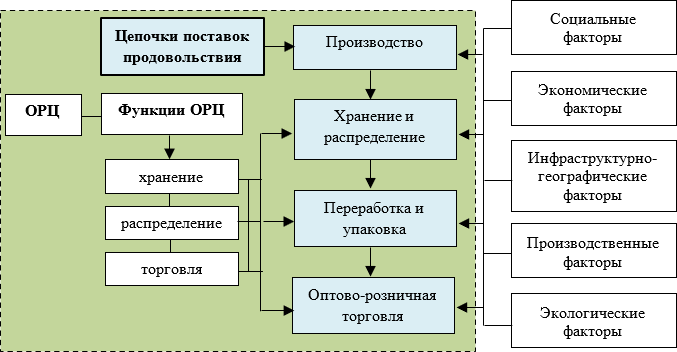
\includegraphics[width=0.8\textwidth]{media/ekon2/image8}
	\caption*{Рис. 1 - Взаимосвязь цепи поставок агропродовольственной продукции и ОРЦ и основные факторы, влияющие на выбор места размещения логистической инфраструктуры}
    \caption*{\normalfont\emph{Примечание -- Разработано автором на основании анализа источников {[}14 -- 17, 32 - 36{]}}}
\end{figure}

\begin{multicols}{2}
Оптимальность размещения может быть определена затратами на реализацию
конечной продукции {[}28{]}. Эффективность может быть определена через
применение следующих показателей: получение прибыли на одного
товаропроизводителя, рентабельность производства и реализации продукции
{[}3{]}, удельный вес убыточных предприятий, входящих в товаропроводящую
сеть.

\emph{Инфраструктурно-географические факторы}. характеризуют потенциал и
способность переработать, производить и реализовывать через сеть
продукцию. Их показатели: численность предприятий и цехов по переработке
и производству агропродовольственной продукции, наличие мощностей для
хранения продукции, торговые площади, численность торговых сетей,
складская площадь, протяженность автомобильных дорог, расстояние от
райцентра до областного центра на автомобильном транспорте, время
проезда на автотранспорте, обеспеченность инженерной и
телекоммуникационной инфраструктурой, плотность автомобильных и железных
дорог {[}16, 32 - 34{]} и др.

\emph{Производственные факторы} включают объемные показатели
производства и реализации сельскохозяйственной продукции {[}35{]}.

\emph{Экологические факторы} характеризуются объемом твердых отходов при
реализации продукции {[}19{]}, выбросами в атмосферу загрязняющих
веществ {[}36{]}.

Такое выделение связано с наличием соответствующего элемента в структуре
системы. Каждый из этих факторов, в конечном итоге, влияет на
эффективность и конкурентоспособность РЦ, надежность, устойчивость и
качество обслуживания.

Следует отметить, что выбор местоположения логистических объектов
зависит не только от вышеназванных факторов, но также и от их
функционального назначения, которые не были рассмотрены в указанных
работах.

С точки зрения устойчивости, наряду с экономическими факторами,
экологическими и социальными аспектами важны также географические и
транспортные возможности региона, являющиеся важными критериями для
выбора места расположения ЛЦ {[}16{]}, что было учтено в наших
исследованиях.

{\bfseries Результаты и обсуждение.} Отсутствие методологических подходов и
рекомендаций по развитию логистической инфраструктуры регионов
определило проблему, поставленную в рамках данной статьи, главная идея
которой состоит в разработке методологического подхода по решению задачи
эффективного размещения объектов логистической инфраструктуры
агропродовольственной продукции на территории регионов Казахстана.

Построение модели ОРЦ агропродовольственной продукции проводится в
последовательности, включающей следующие этапы.

\emph{Этап 1.} Определение потенциальных мест размещения ОРЦ

1.1. Анализ и отбор показателей, определяющих места выбора и размещения

1.2. Стандартизация показателей

1.3. Определение весовых коэффициентов показателей

1.4. Факторный анализ показателей и выявление наиболее важных факторов

1.5. Кластерный анализ для выявления территориального распределения
производств продукций АПК и формирование кластеров

1.6. Расчет рейтингов и дифференциация районов по уровню
привлекательности размещения логистических инфраструктур

\emph{Этап 2.} Уточнение потенциальных мест размещения

2.1. Определение радиуса действия логистической инфраструктуры

2.2. Определение потенциальных мест размещения

\emph{Этап 3.} Определение зоны обслуживания

3.1. Определение зоны обслуживания ОРЦ

3.2. Экономическая интерпретация полученных результатов

\emph{1 этап. Определение потенциальных мест размещения ОРЦ}

На этом этапе определяются потенциально возможные места размещения РЦ на
основе выбранных критериев, анализа производства сельскохозяйственной
продукции на территории каждого района и городских агломераций, а также
сложившейся схемы транспортных путей, размещения объектов логистической
и транспортной (железнодорожного и автомобильного транспорта)
инфраструктуры.

Выбор критериев размещения и определения потребности в объектах
логистической инфраструктуры на примере ОРЦ проводится в следующей
последовательности.

1.1 Анализ и отбор показателей, определяющих места выбора и размещения по
статистическим данным за определенный промежуток времени.

На основе теоретического анализа, исходя из цели исследования, для
характеристики ОРЦ, из литературных источников выбираются показатели,
прямо или косвенно влияющие на выбор места размещения логистических
объектов по статистическим данным Бюро национальной статистики
Республики Казахстан (БНС РК). Вычисление корреляционной матрицы для
переменных, участвующих в анализе, позволяет исключить зависимые
(коррелирующие) параметры, отобрать наиболее значимые факторы.
Оценивается значимость показателей и исключаются незначимые факторы.

1.2. Приведение показателей к стандартному виду, в связи с
неравнозначностью их измерения.

Стандартизация показателей, с целью приведения неравнозначных значений
показателей к однородным значениям, необходима для сравнения
показателей, имеющих разные единицы измерения. Размерность матрицы
определяется как \emph{n*m}, где n -- количество объектов наблюдения, а
m -- количество элементарных признаков.

Осуществляется переход от матрицы исходных данных (\emph{x}) размерности
(n х m) к матрице стандартизированных показателей (\emph{z}) размерности
(n х m). При пересчете всех элементов матрицы в стандартизированный вид
используется формула (1) следующего вида:

\begin{equation}
Z_{ij}=\frac{x_{ij}-x_j}{\sigma_j},
\end{equation}

где \emph{x}\textsubscript{ij} -- \emph{i-}элемент \emph{j-}наблюдения;

𝑥\textsubscript{j}-- среднее значение \emph{i-}элементов
\emph{j-}наблюдения;

𝜎j -- среднее отклонение \emph{i-}элементов \emph{j -} наблюдения.

1.3. Определение весовых коэффициентов показателей позволяет определить
их значимость для формирования рейтинга.

1.4. Проведение факторного анализа с целью выявления наиболее важных
факторов.

Факторный анализ позволяет формировать, сократить количество переменных
и группировать их. На основе анализа строятся матрицы значений факторов
\emph{F\textsubscript{ji}} для всех n территорий (районов, городских
агломераций), которые в дальнейшем используются для расчета рейтинга
места размещения логистических объектов.

1.5. Проведение кластерного анализа на основе \emph{k}-средних,
формирование кластеров.

Для изучения территориального распределения сельскохозяйственного
производства районы Казахстана разбиваются на группы с помощью метода
кластерного анализа.

1.6. Расчет рейтингов и определение интегрального показателя,
дифференциация районов по уровню рейтингового значения.

Расчет самого рейтинга проводится по формуле (2):

\(R_{i\ } = \ \frac{\sum_{i = 1}^{n}F_{ji}}{\ \sum_{i = 1}^{n}b_{nji}},\)
(2)

где 𝑅𝑖 - интегральный показатель привлекательности расположения ОРЦ
\emph{i-} региона, \emph{Fji -} значение \emph{j-}го фактора \emph{i}-го
региона, \emph{n} -- количество факторов,\({\ \ \ \ \ \ b}_{nji\ }\)-
весовой коэффициент \emph{n} показателя \emph{j} фактора \emph{i}
региона.

Полученный в ходе расчета интегральный показатель ранжируется от
наивысшего числа к наименьшему. Высокий балл рейтинга свидетельствует о
потенциальной привлекательности размещения в регионе.

\emph{Этап 2. Уточнение потенциальных мест размещения}

На втором этапе проводится корректировка потенциальных мест размещения
логистических интегрированных РЦ на территории регионов с помощью метода
центра тяжести -- исходя из районов концентрации производства
сельскохозяйственной продукции, транспортной доступности и других
технико-экономических параметров, консолидированных в одном месте.

2.1. Определение радиуса действия торговой инфраструктуры.

На данном этапе проводится расчет радиуса действия ОРЦ с использованием
метода «центра тяжести» {[}37{]}.

2.2. Определение потенциальных мест размещения ОРЦ.

Определение потенциальных мест размещения проводится на основе
факторного анализа матрицы значений \emph{F\textsubscript{i}}.
Определяется среднее значение \emph{F\textsubscript{i}} каждого из
\emph{n} территорий. Выбор видов ОРЦ осуществляется по отдельно
сгруппированным факторным нагрузкам \emph{F\textsubscript{i}}, которые
влияют на выбор хранения, сбыта и торговли, соответственно. Определяется
их среднее значение для каждого района/города. Потенциальное место
размещения объектов определяется, если их скорректированное на веса
среднее значение \emph{F\textsubscript{i}} больше единицы.

\emph{Этап 3. Определение зоны обслуживания}

3.1. Зоны обслуживания ОРЦ (группы сельскохозяйственных районов)
определяются в соответствии с потенциальными местами размещения на
территории районов и городских агломераций.

3.2. Экономическая интерпретация полученных результатов.

Предложенный методический подход к определению потенциального места
размещения ОРЦ и их количества в зависимости от интегрированных
показателей, представленных факторным анализом, является главным
отличием от существующих. Данный подход позволяет быстро и эффективно
определить потребности, исходя из целевого назначения объекта, повышает
эффективность выбора и размещения логистической инфраструктуры.

Оригинальность методики состоит в том, что она дает возможность
одновременно учесть места размещения ОРЦ в зависимости от их назначения
(для хранения, распределения и торговли) и соответствующих факторов.

Предложенная методика выбора мест размещения транспортно-логистических
мощностей, основанная на учете выявленных социально-экономических и
инфраструктурных факторов, может быть рекомендована при составлении
государственных программ по развитию логистики в регионах, а также
крупным компаниям при принятии решения об инвестировании в логистическую
отрасль.

Методика выбора мест размещения ОРЦ для хранения, распределения и
торговли может быть рекомендована при государственном планировании
развития логистической инфраструктуры регионов страны, а также крупным
компаниям при принятии решения об инвестировании в логистическую
отрасль.

Методика расчета состоит в формировании системы показателей,
характеризующих оптимальность размещения и эффективность использования
элементов логистической инфраструктуры, определении индексов,
свидетельствующих об их изменении во временном интервале, вычислении
агрегированного показателя, представляющего собой среднее значение
индексов.

На основе полученных результатов расчета определяются количество,
потенциальные места размещения, а также зоны обслуживания ОРЦ хранения,
ОРЦ распределения, ОРЦ торговли.

{\bfseries Выводы.} Для решения проблемы создания логистической
инфраструктуры по распределению, хранению и торговле сельхозпродукцией
автором предложен методологический подход, позволяющий формировать
модель и определять месторасположение объектов логистической
инфраструктуры.

В качестве ключевого параметра служит совокупность показателей
социально-экономического, регионального, производственного и
экологических факторов региона.

Методика выбора показателей и размещения объектов логистической
инфраструктуры проводилась на основе расчета интегрального показателя
определения эффективного места размещения, зон обслуживания и их
количества в регионах, с использованием комплекса методов.

Методика выбора мест размещения ОРЦ для хранения, распределения и
торговли может быть рекомендована при государственном планировании
развития логистической инфраструктуры регионов страны, а также крупным
компаниям при принятии решения об инвестировании в логистическую
отрасль.

Использование данной методологии позволяет государственным органам или
частным инвесторам заранее, до принятия решения о проектировании или
модернизации существующих распределительных сетей, просчитать возможные
варианты их оптимального размещения, исходя из плотности населения и
транспортно-логистической и торговой инфраструктуры, экономической и
физической доступности продуктов питания и других факторов, что
позволяет повысить эффективность производства и реализации и
устойчивость цепей поставок агропродовольственной продукции.

Используя данный методологический подход, автор провела исследования по
проектированию размещения логистической инфраструктуры для хранения,
распределения и торговли агропродовольственной продукции, что является
материалом для следующей публикации.

\emph{{\bfseries Финансирование.}} Данное исследование выполнялось в рамках
грантового проекта, финансируемого Комитетом по науке Министерства науки
и высшего образования Республики Казахстан (АР19677634 «Развитие
логистической инфраструктуры и устойчивых цепей поставок скоропортящейся
продовольственной продукции на территории Казахстана», 2023 -- 2025 гг.).
\end{multicols}

\begin{center}
{\bfseries Литература}
\end{center}

\begin{references}
1. Rios J., Linfati R., Morillo-Torres D., Derpich I., Gatica G. Optimal
placement design for picking and packing in distribution centers //
Advances in Mechanical Engineering. -- 2021. -- Vol.13(4). -P 1-7. DOI
10.1177/16878140211010657

2. \href{https://www.webofscience.com/wos/author/record/28556133}{Li
Y}.,\href{https://www.webofscience.com/wos/author/record/32561100}{Liu
X.D}.~and~\href{https://www.webofscience.com/wos/author/record/6098832}{Chen
Y}.
\href{https://www.webofscience.com/wos/woscc/full-record/WOS:000288343900166}{Selection~of~logistics~center~location~using
Axiomatic Fuzzy Set and TOPSIS methodology in~logistics~management} //
\href{https://www.sciencedirect.com/journal/expert-systems-with-applications}{Expert
Systems with Applications}. -- 2011. - Vol.38(6). - P.7901-7908. DOI
10.1016/j.eswa.2010.12.161

3. \href{https://www.webofscience.com/wos/author/record/14795379}{Wang
P},~\href{https://www.webofscience.com/wos/author/record/36107182}{Chen
X.J}.\&~\href{https://www.webofscience.com/wos/author/record/32493117}{Zhang,
X.B}.
\href{https://www.webofscience.com/wos/woscc/full-record/WOS:000830775300005}{Research
on~Location~of~Logistics~Distribution Center Based on K-Means
Clustering Algorithm} //
\href{https://www.researchgate.net/journal/Security-and-Communication-Networks-1939-0122}{Security
and Communication Networks}. -- 2022. -~Vol.8. - P.1-9. DOI
\href{http://dx.doi.org/10.1155/2022/2546429}{10.1155/2022/2546429}

4. Cheng Yh., Zhou Sy. Research of Distribution Center Site Selection
Based on Fuzzy Analytic Hierarchy Process / In book: Qi E., Shen J.,
Dou R. (eds) //Proceedings of the 22nd International Conference on
Industrial Engineering and Engineering Management. -- Paris: Atlantis
Press, 2016. - P.335-342. DOI 10.2991/978-94-6239-177-2\_34

5. Paçacı B., Erol S., Çubuk M.K. Çok modlu taşımacılığa uygun lojistik
merkez yer seçimi için bir öneri: Türkiye uygulaması // Journal of
Polytechnic. -- 2023. -- Vol. 26(2). -- P. 923--928. DOI\\
10.2339/politeknik.1099560.

6. \href{https://sciprofiles.com/profile/693277}{Huang}, Y.,
\href{https://sciprofiles.com/profile/2635021}{Wang} X.~and
\href{https://sciprofiles.com/profile/author/dFBVb3FoaXR6WVFmWlV5M0h1dGNXZz09}{Chen}
H. \href{https://www.mdpi.com/2071-1050/14/24/16409}{Location
Selection for Regional Logistics Center Based on Particle Swarm
Optimization} // Sustainability. - 2022. - Vol. 14(24):16409. DOI
10.3390/su142416409

7. Herlina L., Machfud, Sukardi E.A.
\href{http://www.iemsjl.org/journal/article.php?code=82679}{An
Integrated Production and Distribution Planning Model in Shrimp
Agroindustry Supply Chain} // Industrial Engineering \& Management
Systems. - 2022. - Vol.21(1). - P.1-19.
\href{https://doi.org/10.7232/iems.2022.21.1.001}{DOI
10.7232/iems.2022.21.1.001}

8. Ambrosino D. and Scutella M.G. Distribution network design: New
problems and related models // European Journal of Operational
Research. --2005. -Vol.165(3). -P.610-624. DOI\\
10.1016/j.ejor.2003.04.009

9. Mangiaracina R., Perego A., Song G. A quantitative model to support
strategic distribution network design // Proceedings of the 17th LRN
(Logistics Research Network) Annual Conference. -- Bedford: Cranfield
University, 2012. ISBN \emph{978-1-904564-43-0}

10. Romeijn H.E., Shu J., Teo C.-P. Designing Two-Echelon Supply Network
// European Journal of Operational Research. -- 2007. - Vol.178(2).
-P.449--462. DOI 10.1016/j.ejor.2006.02.016.

11. Копылова, O.A. Методика выбора мест размещения
транспортнологастических центров / O.A. Копылова, А.Н. Рахмангулов //
Актуальные проблемы современной науки, техники и образования:
материалы 69-й межрегиональной научно-технической конференции. -
Магнитогорск : Изд-во Магнитогорс. гос. техн. ун-та им. Г.И.Носова,
2011. - № 1. - С. 13-16.

12. Romeijn H.E., Al-Gwaiz M., Chao X. Capacity Expansion and Cost
Efficiency Improvement in the Warehouse Problem // Naval Research
Logistics. -- 2016. - Vol.63(5). - P.367--373. DOI 10.1002/nav.21703

13. Geunes J., Romeijn H.E., Van Den Heuvel W. Improving the Efficiency of
Decentralized Supply Chains with Fixed Ordering // European Journal of
Operational Research. - 2016. - Vol. 252(3). - P.815-828. DOI
10.1016/j.ejor.2016.02.004

14. Попов П. В., Мирецкий И. Ю., Логинова Е. В.~Эффективное размещение
распределительно-подсортировочных складов на территории региона //
Экономика региона. -2017. - Т. 13, вып. 3. - С. 871-882. DOI
10.17059/2017-3-19

15. Горлова Е.Е. Методический подход к размещению центров распределения
сельскохозяйственной продукции в регионе // Экономика и экологический
менеджмент. -- 2012. - №.1. -- С.16-24. URL:
https://economics.ihbt.ifmo.ru/file/article/6763.pdf (дата обращения
19.09.2024).

16. Попов П.В., Мирецкий И.Ю.
\href{https://economyofregion.ru/arhiv/2019-2/nomer-2-2019/metodologiya-postroeniya-logisticheskoj-infrastruktury-na-territorii-regiona/}{Методология
построения логистической инфраструктуры на территории региона} //
Экономика региона. - 2019. - Т. 15, вып. 2. - С. 483-492. DOI
10.17059/2019-2-13

17. \href{https://www.scopus.com/authid/detail.uri?origin=resultslist&authorId=55624611200&zone=}{Eslamipoor
R.}\href{https://www.scopus.com/record/display.uri?eid=2-s2.0-85146138004&origin=resultslist&sort=plf-f&src=s&st1=logistics+center&sid=608c0e84c46c21631ea70ffcaa21b2a6&sot=b&sdt=b&sl=23&s=TITLE\%28logistics+center\%29&relpos=0&citeCnt=0&searchTerm=}{A
two-stage stochastic planning model for locating product collection
centers in green logistics networks} //
\href{https://www.scopus.com/sourceid/21101098869?origin=resultslist}{Cleaner
Logistics and Supply Chain}. -- 2023. -
\href{https://www.sciencedirect.com/journal/cleaner-logistics-and-supply-chain/vol/6/suppl/C}{Vol.6}:
100091 \href{https://doi.org/10.1016/j.clscn.2022.100091}{DOI\\
10.1016/j.clscn.2022.100091}

18. Keleş N., Pekkaya M. Evaluation of logistics centers in~terms of
sustainability via~MCDM methods
//~\href{https://www.emerald.com/insight/publication/issn/0972-7981}{Journal
of Advances in Management Research}. -- 2023. - Vol.20(2).
-P.291-309.~ DOI 10.1108/JAMR-04-2022-0087

19. Wang Y., Li Y., Lu C. Evaluating the Effects of Logistics Center
Location: An Analytical Framework for Sustainable Urban Logistics //
Sustainability. -- 2023. -- Vol. 15(4):3091. DOI 10.3390/su15043091.

20. Orjuela-Castro J.A., Orejuela-Cabrera J.P., Adarme-Jaimes W. Logistics
Network Configuration for Seasonal Perishable Food Supply Chains //
Journal of Industrial Engineering and Management (JIEM). -- 2021.
--Vol. 14(2). --P. 135-151. DOI 10.3926/jiem.3161.

21. Lu L.,Qin J. Multi-regional logistics center location algorithm based
on improved K-means clustering // Computer system application. --
2019. - Vol.28(8). - P. 251--255.

22. Musolino G., Rindone C., Polimeni A., Vitetta A. Planning urban
distribution center location with variable restocking demand
scenarios: General methodology and testing in a medium-size town //
Transport Policy. -- 2019. --Vol. 80. -- P. 157-166. DOI
10.1016/j.tranpol.2018.04.006.

23. Ozmen M.Ё. and Aydogan E.K. Robust multi-criteria decision making
methodology for real life logistics center location problem
//Artificial Intelligence Review. -- 2020. - Vol.53. - P.725-751. DOI
\href{https://link.springer.com/article/10.1007/s10462-019-09763-y}{10.1007/s10462-019-09763-y}

24. Yang Y. Analysis of Influencing Factors of Logistics Center Location
Based on Comprehensive Quality Training // 2019 4th International
Symposium on Management, Economics, E-business and Marketing (ISMEEM
2019). --UK: Francis Academic Press, 2019. --P. 30-34. DOI
10.25236/ismeem.2019.006.

25. Lei H., Li S. An improved algorithm of D-S evidence fusion // Journal
of Physics: Conference Series. 2021. Vol. 1871(1): 012108. DOI
10.1088/1742-6596/1871/1/012108

26. Mieczyґnska M. and Czarnowski I. K-means clustering for SAT-AIS data
analysis // WMU Journal of Maritime Affairs. - 2021. - Vol. 20. -
P.377-400. DOI 10.1007/s13437-021-00241-3

27. \href{https://www.emerald.com/insight/search?q=Riccardo\%20Mangiaracina}{Mangiaracina
R.},~\href{https://www.emerald.com/insight/search?q=Guang\%20Song}{Song
G.}~and~\href{https://www.emerald.com/insight/search?q=Alessandro\%20Perego}{Perego
A.} Distribution network design: a literature review and a research
agenda
//~\href{https://www.emerald.com/insight/publication/issn/0960-0035}{International
Journal of Physical Distribution \& Logistics Management}. -- 2015. -
Vol.45(5). - P.506-531. DOI
\href{http://dx.doi.org/10.1108/IJPDLM-02-2014-0035}{10.1108/IJPDLM-02-2014-0035}

28. Onstein A.T.C., Tavasszy L.A., van Damme D.A. Factors determining
distribution structure decisions in logistics: a literature review and
research agenda // Transport Reviews. -- 2019. - Vol.39(2). -
P.243-260. DOI 10.1080/01441647.2018.1459929

29. \href{https://www.webofscience.com/wos/author/record/24657901}{Kendi
S}.,
\href{https://www.webofscience.com/wos/author/record/13850822}{Radjef
M.S}.,
\href{https://www.webofscience.com/wos/author/record/29644444}{Hammoudi
A}.
\href{https://www.webofscience.com/wos/woscc/full-record/WOS:000598477800004}{Optimization
of agri-food product distribution networks: \\Modeling and application}
// New Medit. -- 2020. - Vol.19(4). - P. 51-68. DOI 10.30682/nm2004d

30. Prataviera L.B. \& Melacini M. Designing global trade and logistics
channels: a focus on the Chinese food and beverage market //
International Journal of Logistics Systems and Management. -- 2023. -
Vol. 44(2). - P.198-225. DOI 10.1504/IJLSM.2023.129001

31. Kuzman B., Prdić N., Dobraš Z. The importance of the wholesale markets
for trade in agricultural products // Economics of Agriculture. -2017.
- Vol.(64)3. -P. 1177-1190.
\href{https://doi.org/10.5937/ekoPolj1703177K}{DOI
10.5937/ekoPolj1703177K}

32. Wiederer C., Straube F. A decision tool for policymakers to foster
higher-value perishable agricultural exports // Transportation
Research Interdisciplinary Perspectives. -- 2019. - Vol.2: 100035.
\href{https://doi.org/10.1016/j.trip.2019.100035}{DOI\\
10.1016/j.trip.2019.100035}

33. \href{https://www.webofscience.com/wos/author/record/34283995}{Banerjee
A}.,~\href{https://www.webofscience.com/wos/author/record/7546927}{Duflo
E}.~\&~\href{https://www.webofscience.com/wos/author/record/27141385}{Qian
N}. On the road: Access to transportation infrastructure and economic
growth in China // Journal of Development Economics. -- 2020. -
Vol.145: 102442.
\href{https://doi.org/10.1016/j.jdeveco.2020.102442}{DOI\\
10.1016/j.jdeveco.2020.102442}

34. \href{https://www.webofscience.com/wos/author/record/1406264}{Nekrasenko
L}.,~\href{https://www.webofscience.com/wos/author/record/30670921}{Pittman
R}.
\&~\href{https://www.webofscience.com/wos/author/record/29112586}{Doroshenko
A}.
\href{https://www.webofscience.com/wos/woscc/full-record/WOS:000530138400006}{Grain
logistics in Ukraine:~the~main challenges and effective ways to reach
sustainability} // \href{javascript:void(0)}{Economic Annals-XXI}. --
2019. -Vol.178(7-8). - P.70-83. DOI 10.21003/ea.V178-06

35. \href{https://www.webofscience.com/wos/author/record/34864370}{Feng
Y.Q}.,~\href{https://www.webofscience.com/wos/author/record/33997583}{Liu
Y.K}.,~\href{https://www.webofscience.com/wos/author/record/34807908}{Chen
Y.J}.
\href{https://www.webofscience.com/wos/woscc/full-record/WOS:000859686100002}{Distributionally
robust~location-allocation models of distribution centers for fresh
products with uncertain demands} //
\href{https://www.sciencedirect.com/journal/expert-systems-with-applications}{Expert
Systems with Applications}. -2022. -Vol.209 (2) :118180.
\href{https://doi.org/10.1016/j.eswa.2022.118180}{DOI
10.1016/j.eswa.2022.118180}

36. Uyanik C., Tuzkaya G., Kalender Z.T., Oguztimur S. An integrated
DEMATEL--IF-TOPSIS \\methodology for logistics centers' location
selection problem: an application for Istanbul Metropolitan area //
Transport. -2020. -Vol.35(6). -P.548-556.
\href{https://doi.org/10.3846/transport.2020.12210}{DOI
10.3846/transport.2020.12210}

37. Geoffrion A.M., Morris J., Webster S. Distribution System Design //
Facility Location: A Survey of Applications and Methods / Ed. Z.
Drezner. -New York: Springer, 1995.- 572 p. ISBN 0387945458.
\end{references}

\begin{center}
{\bfseries References}
\end{center}

\begin{references}
1. Rios J., Linfati R., Morillo-Torres D., Derpich I., Gatica G. Optimal
placement design for picking and packing in distribution centers //
Advances in Mechanical Engineering. -- 2021. -- Vol.13(4). -P 1-7. DOI
10.1177/16878140211010657

2. \href{https://www.webofscience.com/wos/author/record/28556133}{Li
Y}.,\href{https://www.webofscience.com/wos/author/record/32561100}{Liu
X.D}.,\href{https://www.webofscience.com/wos/author/record/6098832}{Chen
Y}.
\href{https://www.webofscience.com/wos/woscc/full-record/WOS:000288343900166}{Selection
of logistics center location using Axiomatic Fuzzy Set and TOPSIS
methodology in~logistics~management} //
\href{https://www.sciencedirect.com/journal/expert-systems-with-applications}{Expert
Systems with Applications}. -- 2011. - Vol.38(6). - P.7901-7908. DOI
10.1016/j.eswa.2010.12.161

3. \href{https://www.webofscience.com/wos/author/record/14795379}{Wang
P},~\href{https://www.webofscience.com/wos/author/record/36107182}{Chen
X.J}.\&~\href{https://www.webofscience.com/wos/author/record/32493117}{Zhang,
X.B}.
\href{https://www.webofscience.com/wos/woscc/full-record/WOS:000830775300005}{Research
on~Location~of~Logistics~Distribution Center Based on K-Means
Clustering Algorithm} //
\href{https://www.researchgate.net/journal/Security-and-Communication-Networks-1939-0122}{Security
and Communication Networks}. -- 2022. -~Vol.8. - P.1-9. DOI
\href{http://dx.doi.org/10.1155/2022/2546429}{10.1155/2022/2546429}

4. Cheng Yh., Zhou Sy. Research of Distribution Center Site Selection
Based on Fuzzy Analytic Hierarchy Process / In book: Qi E., Shen J.,
Dou R. (eds) //Proceedings of the 22nd International Conference on
Industrial Engineering and Engineering Management. -- Paris: Atlantis
Press, 2016. - P.335-342. DOI 10.2991/978-94-6239-177-2\_34

5. Paçacı B., Erol S., Çubuk M.K. Çok modlu taşımacılığa uygun lojistik
merkez yer seçimi için bir öneri: Türkiye uygulaması // Journal of
Polytechnic. -- 2023. -- Vol. 26(2). -- P. 923--928. DOI\\
10.2339/politeknik.1099560.

6. \href{https://sciprofiles.com/profile/693277}{Huang}, Y.,
\href{https://sciprofiles.com/profile/2635021}{Wang} X.~and
\href{https://sciprofiles.com/profile/author/dFBVb3FoaXR6WVFmWlV5M0h1dGNXZz09}{Chen}
H. \href{https://www.mdpi.com/2071-1050/14/24/16409}{Location
Selection for Regional Logistics Center Based on Particle Swarm
Optimization} // Sustainability. - 2022. - Vol. 14(24):16409. DOI
10.3390/su142416409

7. Herlina L., Machfud, Sukardi E.A.
\href{http://www.iemsjl.org/journal/article.php?code=82679}{An
Integrated Production and Distribution Planning Model in Shrimp
Agroindustry Supply Chain} // Industrial Engineering \& Management
Systems. - 2022. - Vol.21(1). - P.1-19.
\href{https://doi.org/10.7232/iems.2022.21.1.001}{DOI
10.7232/iems.2022.21.1.001}

8. Ambrosino D. and Scutella M.G. Distribution network design: New
problems and related models // European Journal of Operational
Research. --2005. -Vol.165(3). -P.610-624. DOI\\
10.1016/j.ejor.2003.04.009

9. Mangiaracina R., Perego A., Song G. A quantitative model to support
strategic distribution network design // Proceedings of the 17th LRN
(Logistics Research Network) Annual Conference. -- Bedford: Cranfield
University, 2012. ISBN \emph{978-1-904564-43-0}

10. Romeijn H.E., Shu J., Teo C.-P. Designing Two-Echelon Supply Network
// European Journal of Operational Research. -- 2007. - Vol.178(2).
-P.449--462. DOI 10.1016/j.ejor.2006.02.016.

11. Kopylova, O.A. Metodika vybora mest razmeshhenija
transportnologasticheskih centrov / O.A. \\Kopylova, A.N. Rahmangulov //
Aktual' nye problemy sovremennoj nauki, tehniki i
obrazovanija: materialy 69-j mezhregional' noj
nauchno-tehnicheskoj konferencii. - Magnitogorsk : Izd-vo Magnitogors.
gos. tehn. un-ta im. G.I.Nosova, 2011. - № 1. - S. 13-16. {[}in
Russian{]}

12. Romeijn H.E., Al-Gwaiz M., Chao X. Capacity Expansion and Cost
Efficiency Improvement in the Warehouse Problem // Naval Research
Logistics. -- 2016. - Vol.63(5). - P.367--373. DOI 10.1002/nav.21703

13. Geunes J., Romeijn H.E., Van Den Heuvel W. Improving the Efficiency of
Decentralized Supply Chains with Fixed Ordering // European Journal of
Operational Research. - 2016. - Vol. 252(3). - P.815-828. DOI
10.1016/j.ejor.2016.02.004

14. Popov P. V., Mireckij I. Ju., Loginova E. V. Jeffektivnoe razmeshhenie
raspredelitel' \\no-podsortirovochnyh skladov na
territorii regiona // Jekonomika regiona. -2017. - T. 13, vyp. 3. - S.
871-882. DOI 10.17059/2017-3-19 {[}in Russian{]}

15. 1Gorlova E.E. Metodicheskij podhod k razmeshheniju centrov
raspredelenija sel' skohozjajstvennoj produkcii v
regione // Jekonomika i jekologicheskij menedzhment. -- 2012. - №.1.
-- S.16-24. URL: https://economics.ihbt.ifmo.ru/file/article/6763.pdf
(data obrashhenija 19.09.2024). {[}in Russian{]}

16. Popov P.V., Mireckij I.Ju. Metodologija postroenija logisticheskoj
infrastruktury na territorii regiona // Jekonomika regiona. - 2019. -
T. 15, vyp. 2. - S. 483-492. DOI 10.17059/2019-2-13{[}in Russian{]}

17. \href{https://www.scopus.com/authid/detail.uri?origin=resultslist&authorId=55624611200&zone=}{Eslamipoor
R.}\href{https://www.scopus.com/record/display.uri?eid=2-s2.0-85146138004&origin=resultslist&sort=plf-f&src=s&st1=logistics+center&sid=608c0e84c46c21631ea70ffcaa21b2a6&sot=b&sdt=b&sl=23&s=TITLE\%28logistics+center\%29&relpos=0&citeCnt=0&searchTerm=}{A
two-stage stochastic planning model for locating product collection
centers in green logistics networks} //
\href{https://www.scopus.com/sourceid/21101098869?origin=resultslist}{Cleaner
Logistics and Supply Chain}. -- 2023. -
\href{https://www.sciencedirect.com/journal/cleaner-logistics-and-supply-chain/vol/6/suppl/C}{Vol.6}:
100091 \href{https://doi.org/10.1016/j.clscn.2022.100091}{DOI\\
10.1016/j.clscn.2022.100091}

18. Keleş N., Pekkaya M. Evaluation of logistics centers in~terms of
sustainability via~MCDM methods
//~\href{https://www.emerald.com/insight/publication/issn/0972-7981}{Journal
of Advances in Management Research}. -- 2023. - Vol.20(2).
-P.291-309.~ DOI 10.1108/JAMR-04-2022-0087

19. Wang Y., Li Y., Lu C. Evaluating the Effects of Logistics Center
Location: An Analytical Framework for Sustainable Urban Logistics //
Sustainability. -- 2023. -- Vol. 15(4):3091. DOI 10.3390/su15043091.

20. Orjuela-Castro J.A., Orejuela-Cabrera J.P., Adarme-Jaimes W. Logistics
Network Configuration for Seasonal Perishable Food Supply Chains //
Journal of Industrial Engineering and Management (JIEM). -- 2021.
--Vol. 14(2). --P. 135-151. DOI 10.3926/jiem.3161.

21. Lu L.,Qin J. Multi-regional logistics center location algorithm based
on improved K-means clustering // Computer system application. --
2019. - Vol.28(8). - P. 251--255.

22. Musolino G., Rindone C., Polimeni A., Vitetta A. Planning urban
distribution center location with variable restocking demand
scenarios: General methodology and testing in a medium-size town //
Transport Policy. -- 2019. --Vol. 80. -- P. 157-166. DOI
10.1016/j.tranpol.2018.04.006.

23. Ozmen M.Ё. and Aydogan E.K. Robust multi-criteria decision making
methodology for real life logistics center location problem
//Artificial Intelligence Review. -- 2020. - Vol.53. - P.725-751. DOI
\href{https://link.springer.com/article/10.1007/s10462-019-09763-y}{10.1007/s10462-019-09763-y}

24. Yang Y. Analysis of Influencing Factors of Logistics Center Location
Based on Comprehensive Quality Training // 2019 4th International
Symposium on Management, Economics, E-business and Marketing (ISMEEM
2019). --UK: Francis Academic Press, 2019. --P. 30-34. DOI
10.25236/ismeem.2019.006.

25. Lei H., Li S. An improved algorithm of D-S evidence fusion // Journal
of Physics: Conference Series. 2021. Vol. 1871(1): 012108. DOI
10.1088/1742-6596/1871/1/012108

26. Mieczyґnska M. and Czarnowski I. K-means clustering for SAT-AIS data
analysis // WMU Journal of Maritime Affairs. - 2021. - Vol. 20. -
P.377-400. DOI 10.1007/s13437-021-00241-3

27. \href{https://www.emerald.com/insight/search?q=Riccardo\%20Mangiaracina}{Mangiaracina
R.},~\href{https://www.emerald.com/insight/search?q=Guang\%20Song}{Song
G.}~and~\href{https://www.emerald.com/insight/search?q=Alessandro\%20Perego}{Perego
A.} Distribution network design: a literature review and a research
agenda
//~\href{https://www.emerald.com/insight/publication/issn/0960-0035}{International
Journal of Physical Distribution \& Logistics Management}. -- 2015. -
Vol.45(5). - P.506-531. DOI
\href{http://dx.doi.org/10.1108/IJPDLM-02-2014-0035}{10.1108/IJPDLM-02-2014-0035}

28. Onstein A.T.C., Tavasszy L.A., van Damme D.A. Factors determining
distribution structure decisions in logistics: a literature review and
research agenda // Transport Reviews. -- 2019. - Vol.39(2). -
P.243-260. DOI 10.1080/01441647.2018.1459929

29. \href{https://www.webofscience.com/wos/author/record/24657901}{Kendi
S}.,
\href{https://www.webofscience.com/wos/author/record/13850822}{Radjef
M.S}.,
\href{https://www.webofscience.com/wos/author/record/29644444}{Hammoudi
A}.
\href{https://www.webofscience.com/wos/woscc/full-record/WOS:000598477800004}{Optimization
of agri-food product distribution networks: \\Modeling and application}
// New Medit. -- 2020. - Vol.19(4). - P. 51-68. DOI 10.30682/nm2004d

30. Prataviera L.B. \& Melacini M. Designing global trade and logistics
channels: a focus on the Chinese food and beverage market //
International Journal of Logistics Systems and Management. -- 2023. -
Vol. 44(2). - P.198-225. DOI 10.1504/IJLSM.2023.129001

31. Kuzman B., Prdić N., Dobraš Z. The importance of the wholesale markets
for trade in agricultural products // Economics of Agriculture. -2017.
- Vol.(64)3. -P. 1177-1190.
\href{https://doi.org/10.5937/ekoPolj1703177K}{DOI
10.5937/ekoPolj1703177K}

32. Wiederer C., Straube F. A decision tool for policymakers to foster
higher-value perishable agricultural exports // Transportation
Research Interdisciplinary Perspectives. -- 2019. - Vol.2: 100035.
\href{https://doi.org/10.1016/j.trip.2019.100035}{DOI\\
10.1016/j.trip.2019.100035}

33. \href{https://www.webofscience.com/wos/author/record/34283995}{Banerjee
A}.,~\href{https://www.webofscience.com/wos/author/record/7546927}{Duflo
E}.~\&~\href{https://www.webofscience.com/wos/author/record/27141385}{Qian
N}. On the road: Access to transportation infrastructure and economic
growth in China // Journal of Development Economics. -- 2020. -
Vol.145: 102442.
\href{https://doi.org/10.1016/j.jdeveco.2020.102442}{DOI\\
10.1016/j.jdeveco.2020.102442}

34. \href{https://www.webofscience.com/wos/author/record/1406264}{Nekrasenko
L}.,~\href{https://www.webofscience.com/wos/author/record/30670921}{Pittman
R}.
\&~\href{https://www.webofscience.com/wos/author/record/29112586}{Doroshenko
A}.
\href{https://www.webofscience.com/wos/woscc/full-record/WOS:000530138400006}{Grain
logistics in Ukraine:~the~main challenges and effective ways to reach
sustainability} // \href{javascript:void(0)}{Economic Annals-XXI}. --
2019. -Vol.178(7-8). - P.70-83. DOI 10.21003/ea.V178-06

35. \href{https://www.webofscience.com/wos/author/record/34864370}{Feng
Y.Q}.,~\href{https://www.webofscience.com/wos/author/record/33997583}{Liu
Y.K}.,~\href{https://www.webofscience.com/wos/author/record/34807908}{Chen
Y.J}.
\href{https://www.webofscience.com/wos/woscc/full-record/WOS:000859686100002}{Distributionally
robust~location-allocation models of distribution centers for fresh
products with uncertain demands} //
\href{https://www.sciencedirect.com/journal/expert-systems-with-applications}{Expert
Systems with Applications}. -2022. -Vol.209 (2) :118180.
\href{https://doi.org/10.1016/j.eswa.2022.118180}{DOI
10.1016/j.eswa.2022.118180}

36. Uyanik C., Tuzkaya G., Kalender Z.T., Oguztimur S. An integrated
DEMATEL--IF-TOPSIS \\methodology for logistics centers' location
selection problem: an application for Istanbul Metropolitan area //
Transport. -2020. -Vol.35(6). -P.548-556.
\href{https://doi.org/10.3846/transport.2020.12210}{DOI
10.3846/transport.2020.12210}

37. Geoffrion A.M., Morris J., Webster S. Distribution System Design //
Facility Location: A Survey of Applications and Methods / Ed. Z.
Drezner. -New York: Springer, 1995.- 572 p. ISBN 0387945458.
\end{references}

\begin{authorinfo}
\emph{{\bfseries Сведения об авторе}}

Сыздыкбаева Б.У. -- д.э.н., профессор Евразийского национального
университета имени Л.Н. Гумилева, Астана, Казахстан. e-mail:
bakyt\_syzdykbaeva@mail.ru

\emph{{\bfseries Автор туралы мәліметтер}}

Сыздықбаева Б.Ұ. -- э.ғ.д., Л.Н. Гумилев атындағы Еуразия ұлттық
университетінің профессоры, Астана, Қазақстан. e-mail:
bakyt\_syzdykbaeva@mail.ru

\emph{{\bfseries Information about the author}}

Syzdykbayeva B.U. {\bfseries -} doctor of economic sciences, professor of
L.N. Gumilyov Eurasian National University, Astana, Kazakhstan. e-mail:
bakyt\_syzdykbaeva@mail.ru
\end{authorinfo}
